\beginsong{Molly Malone}[
    wuw={James Yorkston}, 
    jahr={1883}, 
    bo={210}, 
    pfii={205}, 
    kssiv={134}, 
    biest={579}, 
    siru={134}, 
    index={In Dublin's fair city},
]

\beginverse
\endverse
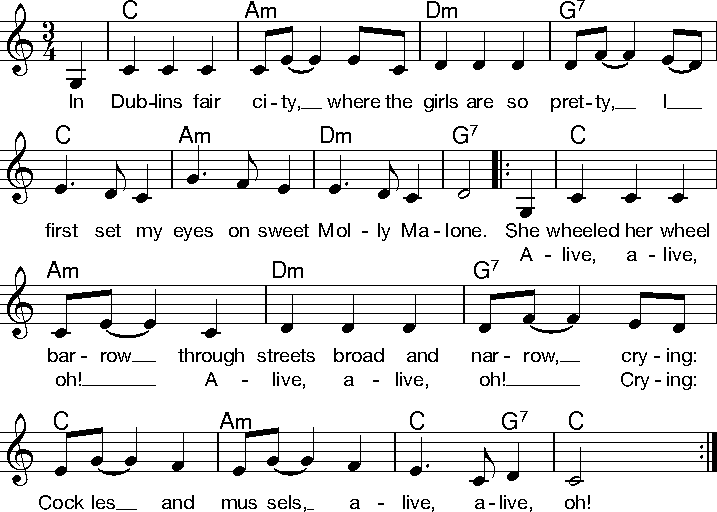
\includegraphics[draft=false, width=1\textwidth]{Noten/Lied066.pdf}

\beginverse
She \[C]was a fish\[Am]monger, which \[Dm]was no \[G7]wonder
for \[C]so was her \[Am]father and \[Dm]mother be\[G7]fore.
And they \[C]both wheeled their bar\[Am]row
through \[Dm]streets broad and \[G7]narrow, crying:
\[C]Cockles and \[Am]mussels, a\[C]live, a\[G7]live, \[C]oh!
A\[C]live, alive, \[Am]oh, a\[Dm]live, alive, \[G7]oh! Crying:
\[C]Cockles and \[Am]mussels, a\[C]live, a\[G7]live, \[C]oh!
\endverse

\beginverse
She ^died of a ^fever and ^no one could ^save her
and ^that was the ^end of sweet ^Molly Ma^lone.
But her ^ghost wheels her ^barrow
through ^streets broad and ^narrow, crying:
^Cockles and ^mussels, a^live, a^live, ^oh!
A^live, alive, ^oh, a^live, alive, ^oh! Crying:
^Cockles and ^mussels, a^live, a^live, ^oh!
\endverse

\endsong

\beginscripture{}
Molly Malone, auch bekannt unter dem Titel ''Cockles and Mussels'' („Herzmuscheln und Miesmuscheln“), ist ein bekanntes irisches Volkslied und eine inoffizielle Hymne der Stadt Dublin. Die Ballade erzählt die Geschichte einer schönen Dubliner Fischhändlerin, die in jungen Jahren an nicht näher bestimmtem Fieber stirbt.
Das Lied wurde auch in der Stanley-Kubrick-Verfilmung von ''A Clockwork Orange'' verwendet: In einer der Schlüsselszenen singt ein betrunkener Landstreicher das Lied.
\endscripture

